
\documentclass[12pt,letterpaper]{article}
\usepackage{amsmath}
\usepackage{amsfonts}
%\usepackage{color}
\usepackage[usenames,dvipsnames]{color}
\usepackage{graphicx}
\usepackage{longtable}
\usepackage{rotating}
\usepackage{verbatim}
\usepackage[pdftex,bookmarksopen]{hyperref}
\hypersetup{pdfauthor={John Sibert}}
\hypersetup{pdfsubject={Compartment model of MHI YFT}}
\hypersetup{pdftitle={Two-compartment models of Main Hawaiian Islands
Yellowfin Tuna Population}}
\hypersetup{pdfkeywords={yellowfin, compartment model, Hawaii}}

\newcommand\doublespacing{\baselineskip=1.6\normalbaselineskip}
\newcommand\singlespacing{\baselineskip=1.0\normalbaselineskip}
\renewcommand\deg[1]{$^\circ$#1}
\newcommand\SD{SEAPODYM}
\newcommand\MFCL{MULTIFAN-CL}
\newcommand\ADMB{ADModel Builder}
\newcommand\SPC{Secretariat of the Pacific Community}
\newcommand\WCPO{Western Central Pacific Ocean}
\newcommand\SSAP{Skipjack Survey and Assessment Programme}
\newcommand\RTTP{Regional Tuna Tagging Programme}
\newcommand\PTTP{Pacific Tuna Tagging Programme}
\newcommand\FAD{fish aggregating device}
\newcommand\ADRM{advection-diffusion-reaction model}
\newcommand\help[1]{\color{Magenta}{\it #1 }\normalcolor}
\newcommand\widebar[1]{\overline{#1}}
\newcommand\EEZ{Exclusive Economic Zone}

\newcommand\None{{N_{1,1}}}
\newcommand\Ntwo{{N_{2,1}}}
\newcommand\Nsum{{N_{1,1}+N_{2,1}}}
\newcommand\peryr{yr$^{-1}$}
\newcommand\prevN[1]{{#1_{t-\Delta t}}}
\newcommand\nextN[1]{{#1_t}}

\title{Two-compartment models of Main Hawaiian Islands Yellowfin Tuna
Population}

\author{
John Sibert\thanks{sibert@hawaii.edu}\\
Joint Institute of Marine and Atmospheric Research\\
University of Hawai'i at Manoa\\
Honolulu, HI  96822 U.S.A.\\[0.125in]
\date{\today}
}

\pagestyle{myheadings}
\markright{Sibert\hfil MHI Comparment Model\hfil{\bf DRAFT}\hfil\today}

\begin{document}
\maketitle

\doublespacing

\section*{Introducetion}
The Yellowfin Tuna (YFT) population in main Hawaiian Islands (MHI) is
embedded in a larger pan-Pacific stock. Nevertheless, local fishermen
believe that the MHI supports a ``resident'' yellowfin population, and
some scientific observations are consistent with this belief. 
Recent tagging, tracking and
studies show that the rate of exchange between the MHI population
and the larger stock is low (Itano and Holland 2000). Analysis
of YFT otoliths sampled from
throughout the Pacific conclude that approximately 90\% of the MHI
population was reared in the MHI (Wells et al 2012).

The Hawaii based deep- and shallow-set longline, inshore- and
offshore- troll and handline components of the fisheries combined catch
approximately 5000 mt of YFT annually (ref). Management of these
fisheries is an important issue deserving of scientific support.

This paper explores some potential models that might be used to
analyze options for the management of fisheries for YFT in the MHI.

\section*{Models}
The principle assumptions for modeling the MHI YFT population are:
\begin{enumerate}
\item The Pacific yellowfin population consists of two components: those
that live in the MHI (region 1) and those that live elsewhere (region
2).
\item Fish immigrate from region 2 to region 1, mix thoroughly, and
interact with the ``resident'' population according to
shared population dynamics.
\item Fish emigrate from region 1 to region 2, but emigrant fish have
no effect on region 2 population dynamics.
\item Immigrant fish are indistinguishable from ``resident'' fish
(i.e. both groups of fish have the same population dynamics) and are
caught by the same gear.
\end{enumerate}

The general modeling approach to be applied will be similar to the
state-space model utilized by Nielsen and Berg (2014). 
State-space models separate variability in the biological
processes in the system (transition model)
 from errors in observing features of interest
in the system (observation model). 
This separation provides some statistical advantages in
estimating model parameters. The models discussed here are potential
candidates for the transition equation in a state-space model.

\subsection*{Logistic population dynamics (Schaefer Model)}
Let $\None$ equal the population size of fish originating in region 1
and residing in region 1
and $\Ntwo$ equal the population size of fish originating in region 2
but residing in region 1.
The total population size of fish residing in region 1 is thus
$\Nsum$, and the dynamics of the population in region 1 is represented as
\begin{equation}
\frac{d}{dt}\big(\Nsum\big)=\big(\Nsum\big)\Big[r\Big(1-\frac{\Nsum}{K}\Big) -F - T_{12}\Big] + T_{21}
\label{eqn:basic}
\end{equation}
where $r$ is the per capita logistic growth rate per year (\peryr), $K$ is the
logistic ``carrying capacity'' measured in the same units as $\None$
and $\Ntwo$, $F$ is the fishing mortality (\peryr) in region 1, and $T_{12}$
is the emigration rate (\peryr) from region 1 to region 2. $T_{21}$
is the annual rate of immigration of fish from region 2 to region 1
measured in the same units as $K$ per year.

Equivalent differential equations could be devised for the dynamics of
fish residing in region 2 (i.e., $\frac{dN_{2,2}}{dt}$ and
$\frac{dN_{1,2}}{dt}$) but 
the dynamics of the fish population in region 2 is external to this
model. $T_{21}$ can be considered to be form of population forcing
from the larger stock in which the MHI population is embedded, perhaps
estimated from other models, such as \MFCL\ or \SD, or perhaps
represented by an
autocorrelated stochastic process. The appearance of
$\Nsum$ in the numerator of the logistic term reflects the assumption
that the population dynamics fish immigrating into region 1 depend on
the population dynamics in region 1. This assumption leads to an
important non-linearity in the model that permits overwhelming of a
local stock by a more numerous immigrant stock as is often characteristics of
mixed-stock fisheries.

The ratio $\frac{\None}{\Nsum}$ is of potential interest, so
equation~\ref{eqn:basic} needs to be expanded and rearranged
leading to a set of simultaneous differential equation for the
components of the population inhabiting region 1.
\begin{eqnarray}
\frac{d\None}{dt}&=&\None\Big[r\Big(1-\frac{\None}{K}\Big)
-F - T_{12}\Big] - \frac{r}{K}T_{12}\None\Ntwo\nonumber\\
\frac{d\Ntwo}{dt}&=&\Ntwo\Big[r\Big(1-\frac{\Ntwo}{K}\Big)
-F - T_{12}\Big] - \frac{r}{K}T_{12}\None\Ntwo + T_{21}
\label{eqn:coupledschaefer}
\end{eqnarray}

The non-linear term from equation~\ref{eqn:basic} appears the term
$\None\Ntwo$ above equations.

The equilibrium of this system can be found by setting
$\frac{d\None}{dt} = 0 = \frac{d\Ntwo}{dt}$. After some simplification
the result is $\frac{T_{21}}{\Ntwo} = 0$ In other words, there is no
equilibrium in this coupled system, other than the degenerate case of
no immigration ($T_{21}=0$) into the MHI. Thus, the notion of using
equilibrium-based reference points such as MSY to manage fisheries for
MHI yellowfin is ill advised.

Example populations trajectories from equationis \ref{eqn:coupledschaefer}
can be seen in figures~\ref{fig:noxfer} through \ref{fig:variance}.
The lack of a steady state caused immigration can be clearly seen in
figure~\ref{fig:emandimm}.
The simulation in figure~\ref{fig:variance} was generated with
correlated normally distributed random variation in both populations
with standard deviation equal to 5\% of the intrinsic growth
rate and correlation coefficient of -0.5. That is, small inversely
correlation random fluctuations were imposed on both populations.
The ratio of emigration to immigration was about 0.1. This result
suggests that random variability may stabilize the population so that a
persistent``local stock'' is maintained.

Equations \ref{eqn:coupledschaefer} are solved by finite difference
approximations using explicit time stepping.
\begin{eqnarray}
\frac{d\None}{dt}\approx\frac{\nextN{\None}-\prevN{\None}}{\Delta t}&=&
\prevN{\None}\Big[r\Big(1-\frac{\prevN{\None}}{K}\Big)
-F - T_{12}\Big]  \nonumber\\
&-& \frac{r}{K}T_{12}\prevN{\None}\prevN{\Ntwo}\\
\frac{d\Ntwo}{dt}\approx\frac{\nextN{\Ntwo}-\prevN{\Ntwo}}{\Delta t}&=&
\prevN{\Ntwo}\Big[r\Big(1-\frac{\prevN{\Ntwo}}{K}\Big)
-F - T_{12}\Big]  \nonumber\\
&-& \frac{r}{K}T_{12}\prevN{\None}\prevN{\Ntwo} + T_{21}
\end{eqnarray}
Rearrangement and addition of process error terms ($\eta_{r,t}$)
yields a form suitable for use as the transition equation in a state-space
model.
\begin{eqnarray}
\nextN{\None}=\Bigg[\prevN{\None}&+&{\Delta t}
\prevN{\None}\Big[r\Big(1-\frac{\prevN{\None}}{K}\Big)
-F - T_{12}\Big]\nonumber\\
&-&\frac{r}{K}T_{12}\prevN{\None}\prevN{\Ntwo}
\Bigg]e^{\eta_{1,t}}\\
\nextN{\Ntwo}=\Bigg[\prevN{\Ntwo}&+&{\Delta t}
\prevN{\Ntwo}\Big[r\Big(1-\frac{\prevN{\Ntwo}}{K}\Big)
-F - T_{12}\Big]\nonumber\\
&-&\frac{r}{K}T_{12}\prevN{\None}\prevN{\Ntwo}
+T_{21}\Bigg]e^{\eta_{2,t}}
\end{eqnarray}
Experience shows that these approximations are sufficiently stable
with reasonably small time steps. 
\help{Is it appropriate to use different process error time series 
($\eta_{1,t}$ and $\eta_{2,t}$) for both
segments of the population under the assumption of identical population
dynamics for both segments?}

\help{Measurement equation needs to be developed.}

\subsection*{General production model (Pella-Tomlinson Model)}
\help{Probably not worth the effort.}

%\clearpage
\subsection*{Age structured model}
\newcommand{\NNone}[2]{N_{1,#1,#2}}
\newcommand{\NNtwo}[2]{N_{2,#1,#2}}
The issue of regulating MHI YFT fisheries by imposing minimum size
limits on some components of the fishery has been raised yet again.
Size- or age-structured models are obviously required to address catch-at-size
issues. The following set of equations are a potential formulation
of the transition equation in a state-space model and are based on the
state-space stock assessment model of Nielsen and Bert (2014). The notation has
been shortened to so that $N_{r,a,t}$ now represents the fish living
in the MHI but originating in in region $r; r = 1,2$ of age $a; a =
1, 2, \ldots, A$ in time interval $t$.
\begin{eqnarray}
\NNone{1}{t}&=&\exp\Big(R\big(\sum_a{p_{a,t-1}(\NNone{a}{t-1}+\NNtwo{a}{t-1})}\big)+\eta_{1,1,t}\Big)\\
\NNtwo{1}{t}&=&T_{2,1,1,t}e^{\eta_{2,1,t}}\\
\nonumber\\
\NNone{a}{t}&=&\NNone{a-1}{t-1}\exp(Z_{a-1,t-1}+\eta_{1,a,t});\qquad 1<a<A \\
\NNtwo{a}{t}&=&\NNtwo{a-1}{t-1}e^{Z_{a-1,t-1}}+T_{2,1,a,t}e^{\eta_{2,a,t}}\\
\nonumber\\
\NNone{A}{t}&=&\Big(\NNone{A-1}{t-1}e^{Z_{A-1,t-1}}+\NNone{A}{t-1}e^{Z_{A,t-1}}\Big)e^{\eta_{1,A,t}}\\
\NNtwo{A}{t}&=&\NNtwo{A-1}{t-1}e^{Z_{A-1,t-1}}+\NNtwo{A}{t-1}e^{Z_{A,t-1}}+T_{2,1,A,t}e^{\eta_{2,A,t}} 
\end{eqnarray}
where $Z_{a,t} = -\sum_gF_{g,a,t} - M_{a} - T_{1,2}$ is a negative quantity
representing the total mortality at fish of age $a$ in time interval
$t$ and
$M_{a}$ is the natural mortality at age $a$, assumed to be constant
over time. 
$F_{g,a,y}$ is the fishing mortality exerted by gear $g$, on fish of
age $a$ during time period $t$. Fishing mortality is usually
represented as the product of several parameters and variables, for
example, catchability coefficient, gear selectivity, and fishing
effort. The parameters of this relationship are often confounded and
difficult to estimate. Furthermore, in the case of MHI yellowfin
fishery, effort estimates are known to be inconsistent, requiring
adjustments to catchability and gear selectivity. Eliminating 
fishing effort would simply the model somewhat.
Fishing mortality is assumed to vary
seasonally (by quarter), to increase or decrease over time, and to
depend on gear selectivity.
\begin{equation}
F_{g,a,t} = e^{-\alpha_{g,Q(t)}}\cdot e^{-\beta_{g,Y(t)}}\cdot S_{g,a,t}
\end{equation}
$\alpha$ is a vector of quarterly deviations from the mean
fishing mortality that sum to zero.
$\beta$ is a vector of autocorrelated annual deviations from the mean
that reflect secular trends in fishing mortality.
$S_{g,a,t}$ represents the selectivity of gear $g$ on age class $a$
fish during time period $t$.
\help{At this point, is is not clear whether
seculare trends in gear efficiency would be best parameterized by
$\beta$ or by $S$.}


%Independent estimates of Pacific YFT natural morality at age are
%available from \MFCL\ (Davies,et al 2014), and estimates of MHI YFT
%natural mortality by size class
%are available from Adam (et al 2003).
%$T_{1,2}$ is the instantaneous transfer rate of
%fish out of the MHI assumed to be independent of age of fish.
%$T_{2,1,a,y}$ is the total rate of transfer of age
%$a$ fish into the MHI in year $y$ which could be parameterized as a simple
%proportion of the numbers at age estimated from \MFCL.

The yield or catch in the MHI under this model would be
\begin{equation}
C_{g,a,t} =
\frac{F_{g,a,t}}{Z_{a,t}}\Big(1-e^{Z_{a,t}}\Big)\Big(\NNone{a}{t}+\NNtwo{a}{t}\Big)e^{\varepsilon_{g,a,t}}
\end{equation}
using the standard Baranov approximation.

\singlespacing
\section*{References}
{\parindent=0cm \small
\everypar={\hangindent=2em \hangafter=1}\par
\doublespacing
Adam, M. S., J. Sibert, D. Itano and K. Holland. 2003. Dynamics of
bigeye (Thunnus obesus) and yellowfin tuna (T. albacares) in Hawaii's
pelagic fishery: analysis of tagging data with a bulk transfer model
incorporating size specific attrition. Fishery Bulletin 101(2):
215-228.

Davies, N., S. Harley, J. Hampton, S. McKechnie. 2014. Stock
assessment of yellowfin tuna in the western and central pacific ocean.
WCPFC-SC10-2014/SA-WP-04.

Itano, D., K. Holland. 2000.  Movement and vulnerability of bigeye
(Thunnus obesus) and yellowfin tuna (Thunnus albacares) in relation to
FADs and natural aggregation points.Aquat. Living Resour. 13: 213-223.

Kleiber, P., J. Hampton, N. Davies, S. Hoyle, D. Fournier. 2014.
MULTIFAN-CL User’s Guide

Nielsen, A. and C. Berg. 2014. Estimation of time-varying selectivity
in stock assessments usingstate-space models. Fisheries Research
158:96-101.

Wells, D., J. Rooker, D. Itano. 2012.  Nursery origin of yellowfin
tuna in the Hawaiian Islands. Mar. Ecol. Prog. Ser. 461:187-196. 
\par}

\clearpage
%%%%%%%% figures begin here %%%%%%%%%%%%%%%%%%%%%%
\begin{figure}
\begin{center}
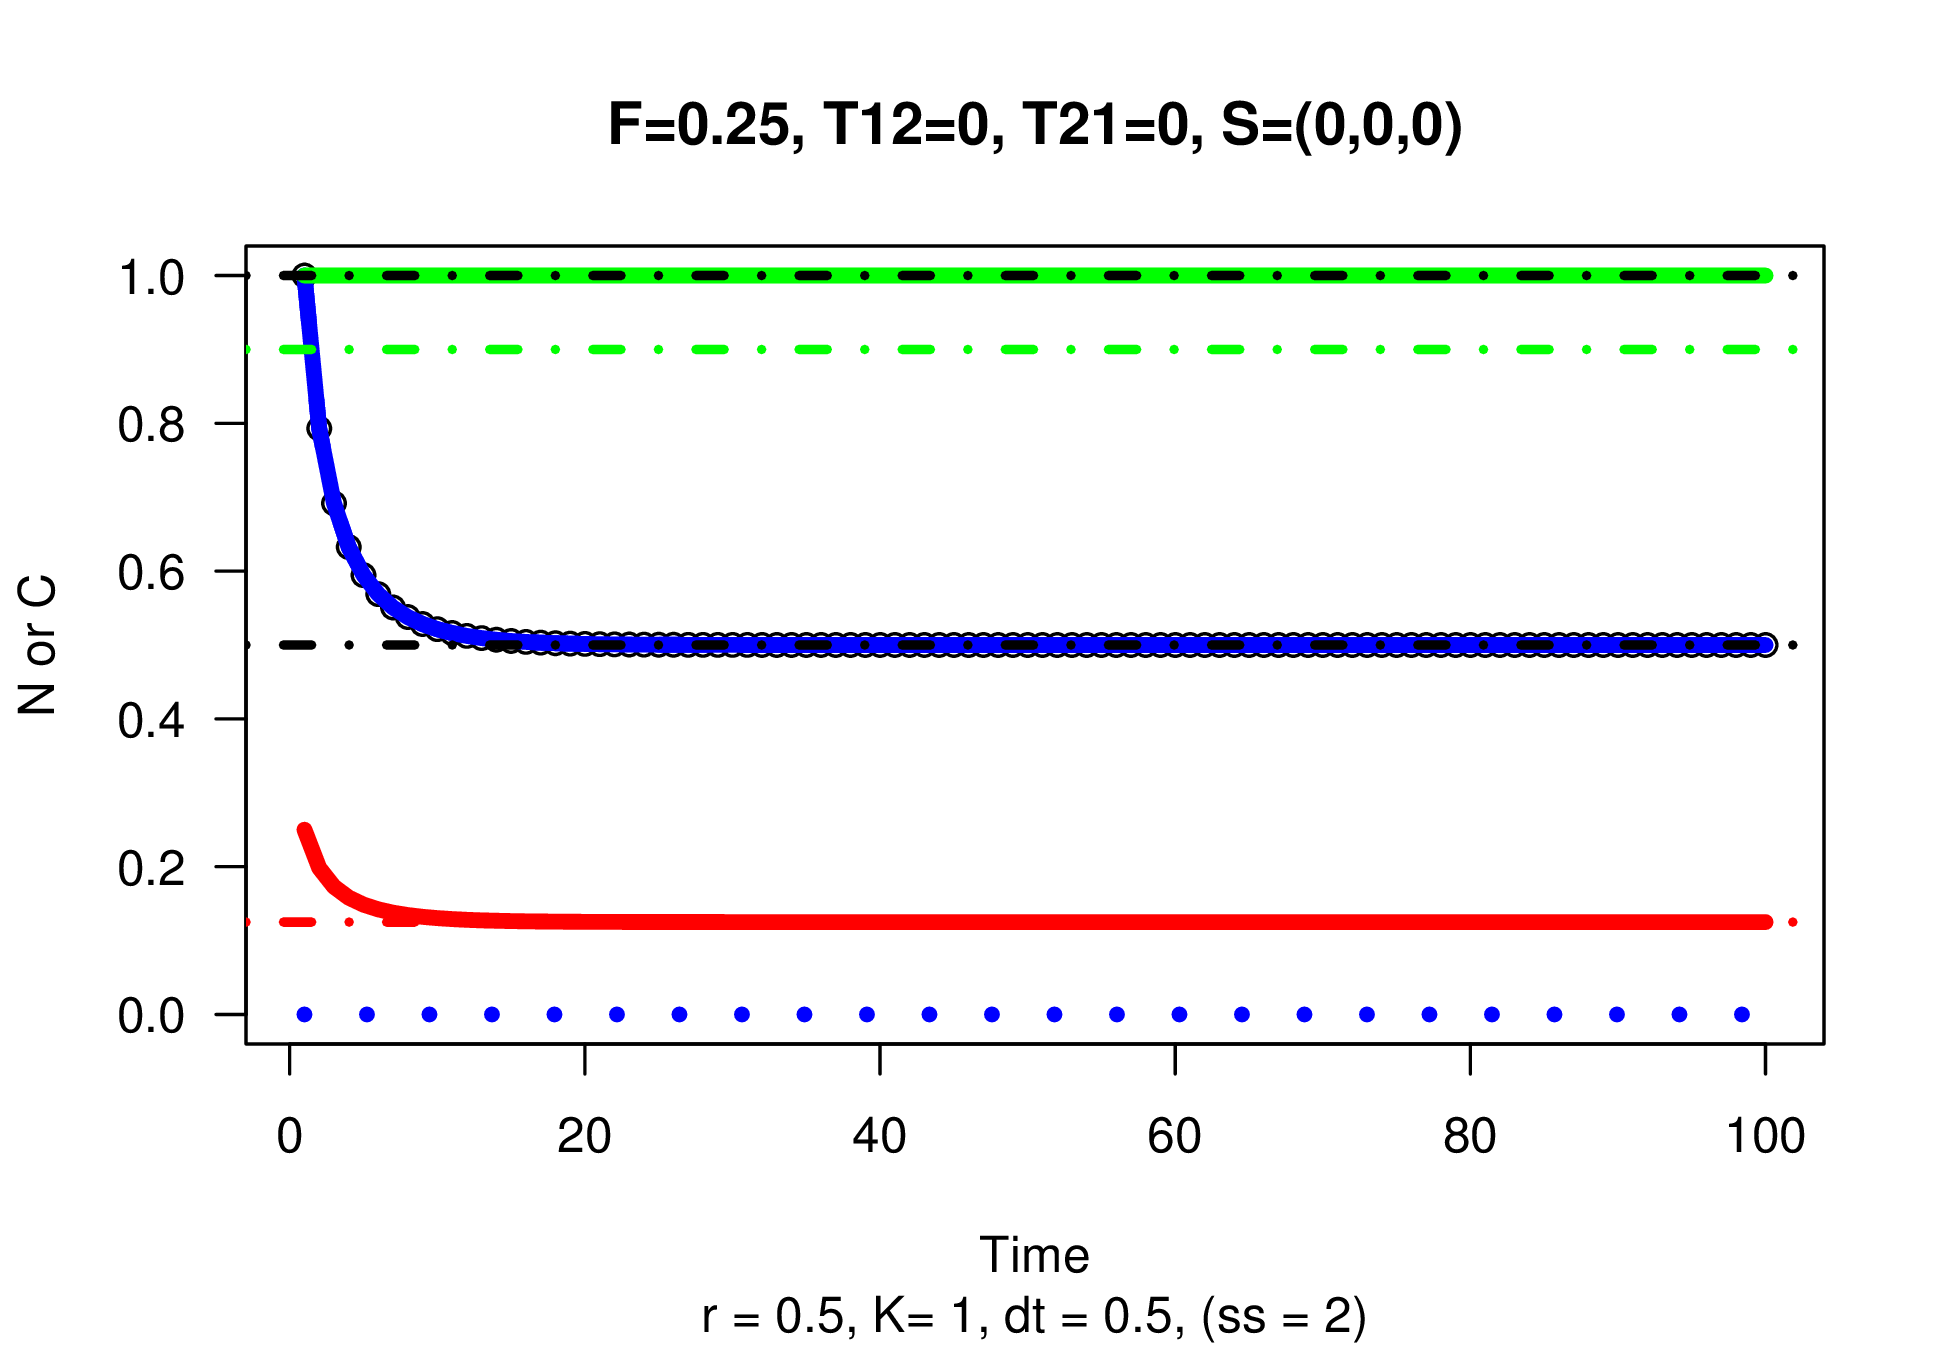
\includegraphics[height=0.7\textwidth]{./graphics/r05F025T120T210S000.png}
\caption{\label{fig:noxfer}
Simple Schaefer model dynamics with no emigration or immigration
($T_{12} = 0 = T_{21}$).
The heavy blue line represents the size of the population ($\Nsum$) moving
from its initial size of 1.0 to its equilibrium size of 0.5
The dashed blue line (in some figures) represents the size of the
$\None$ population.
The dotted blue line represents the size of the $\Ntwo$ population.
The heavy red line represents the yield to the fishery dropping to MSY
(red dash dot line).
The solid green line represents the proportion of ``local'' fish in
the population ($\frac{\None}{\Nsum}$).
The green dash dot line represents the value of the ``proportion
local'' estimated from tagging and ololith analysis.
}
\end{center}
\end{figure}

%\renewcommand{\arraystretch}{0.1}

\begin{figure}
\begin{center}
\begin{tabular}{c}
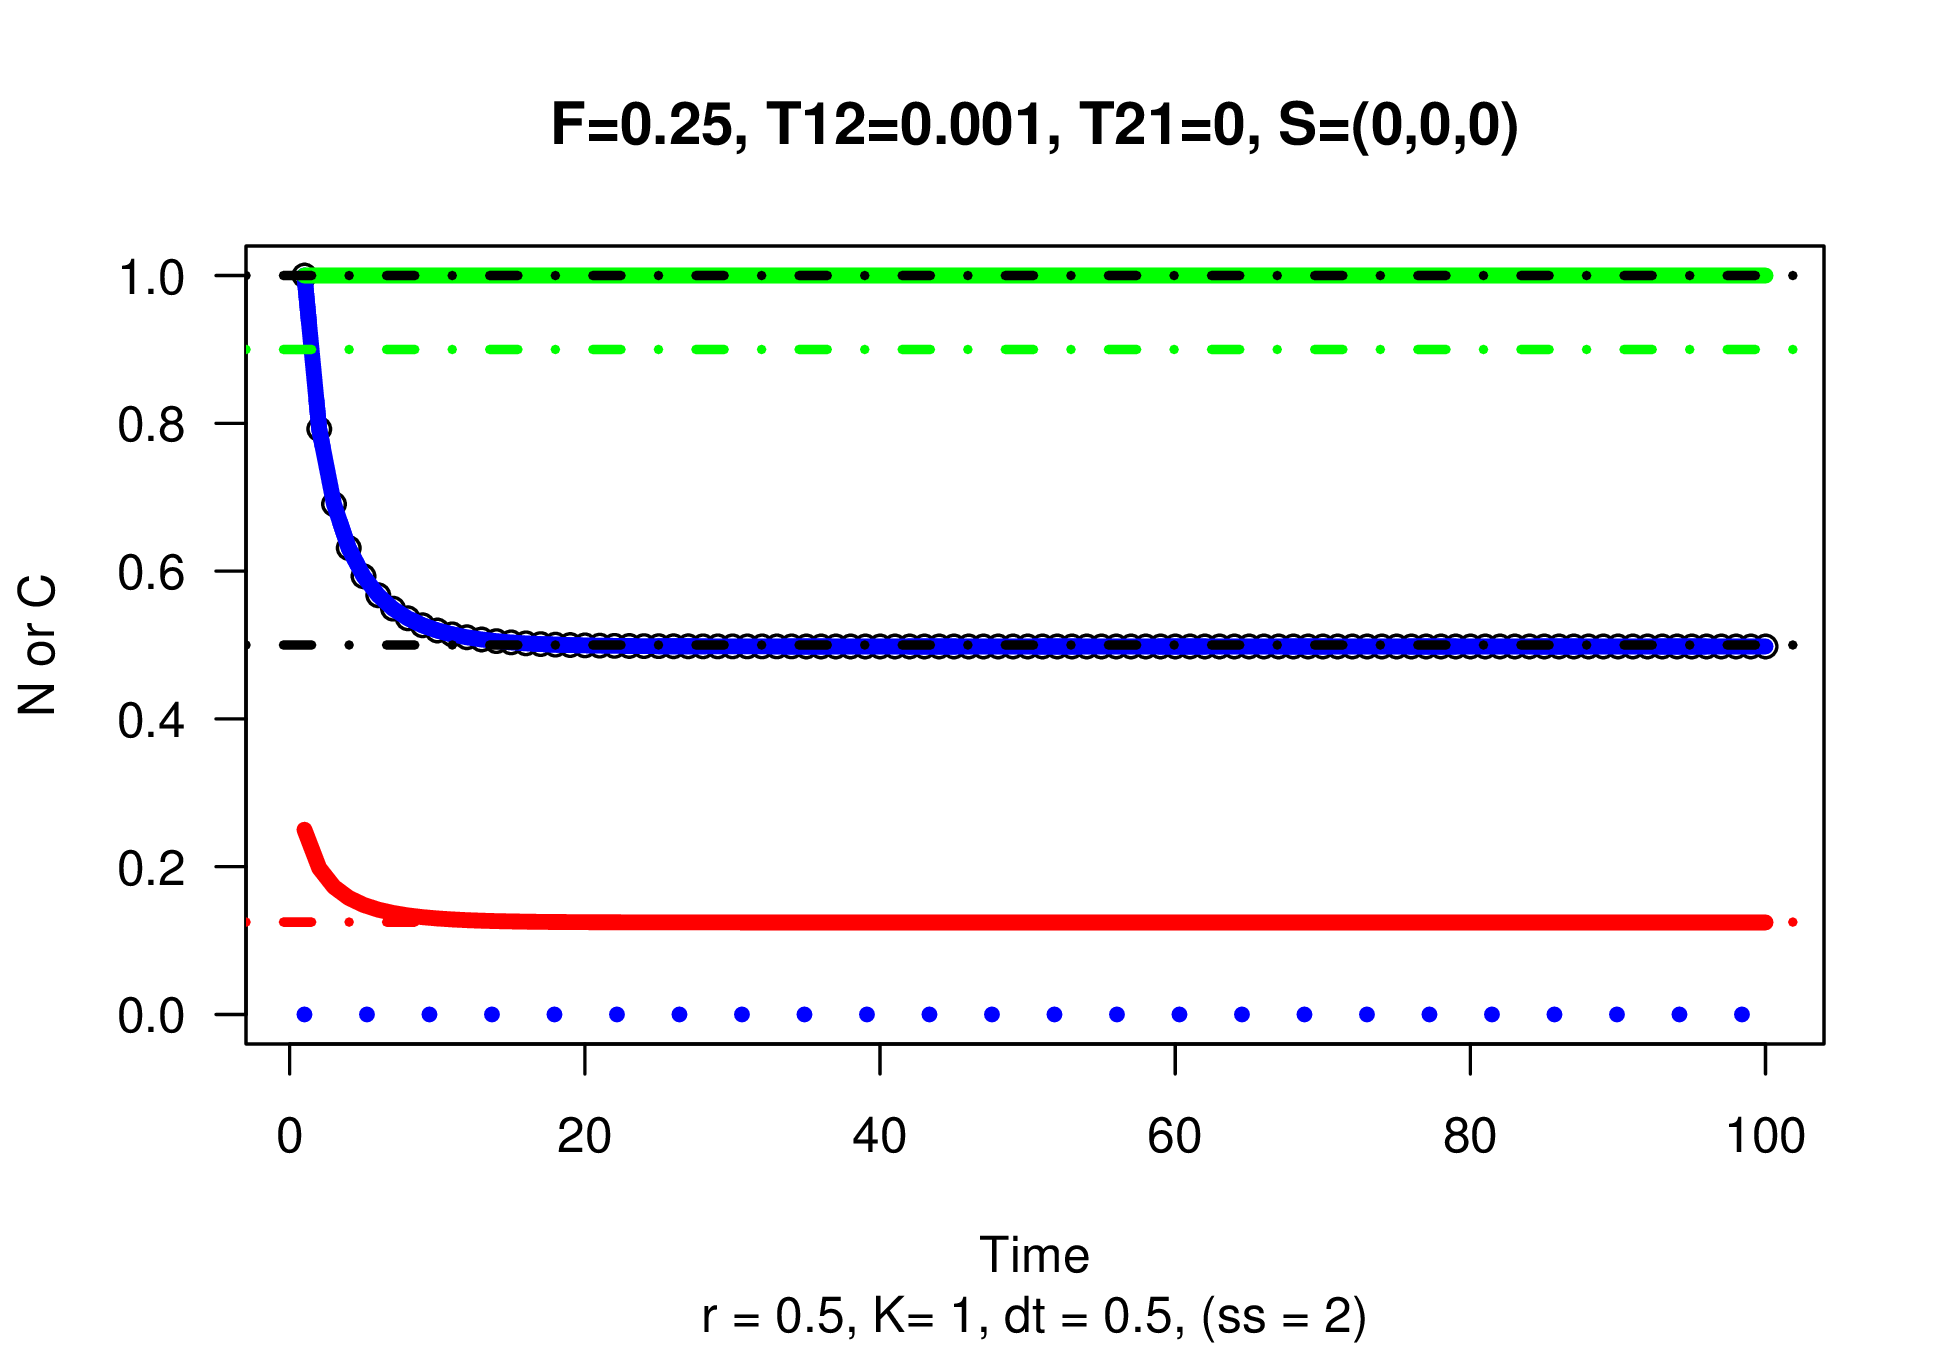
\includegraphics[height=0.5\textwidth]{./graphics/r05F025T120001T210S000.png}\\
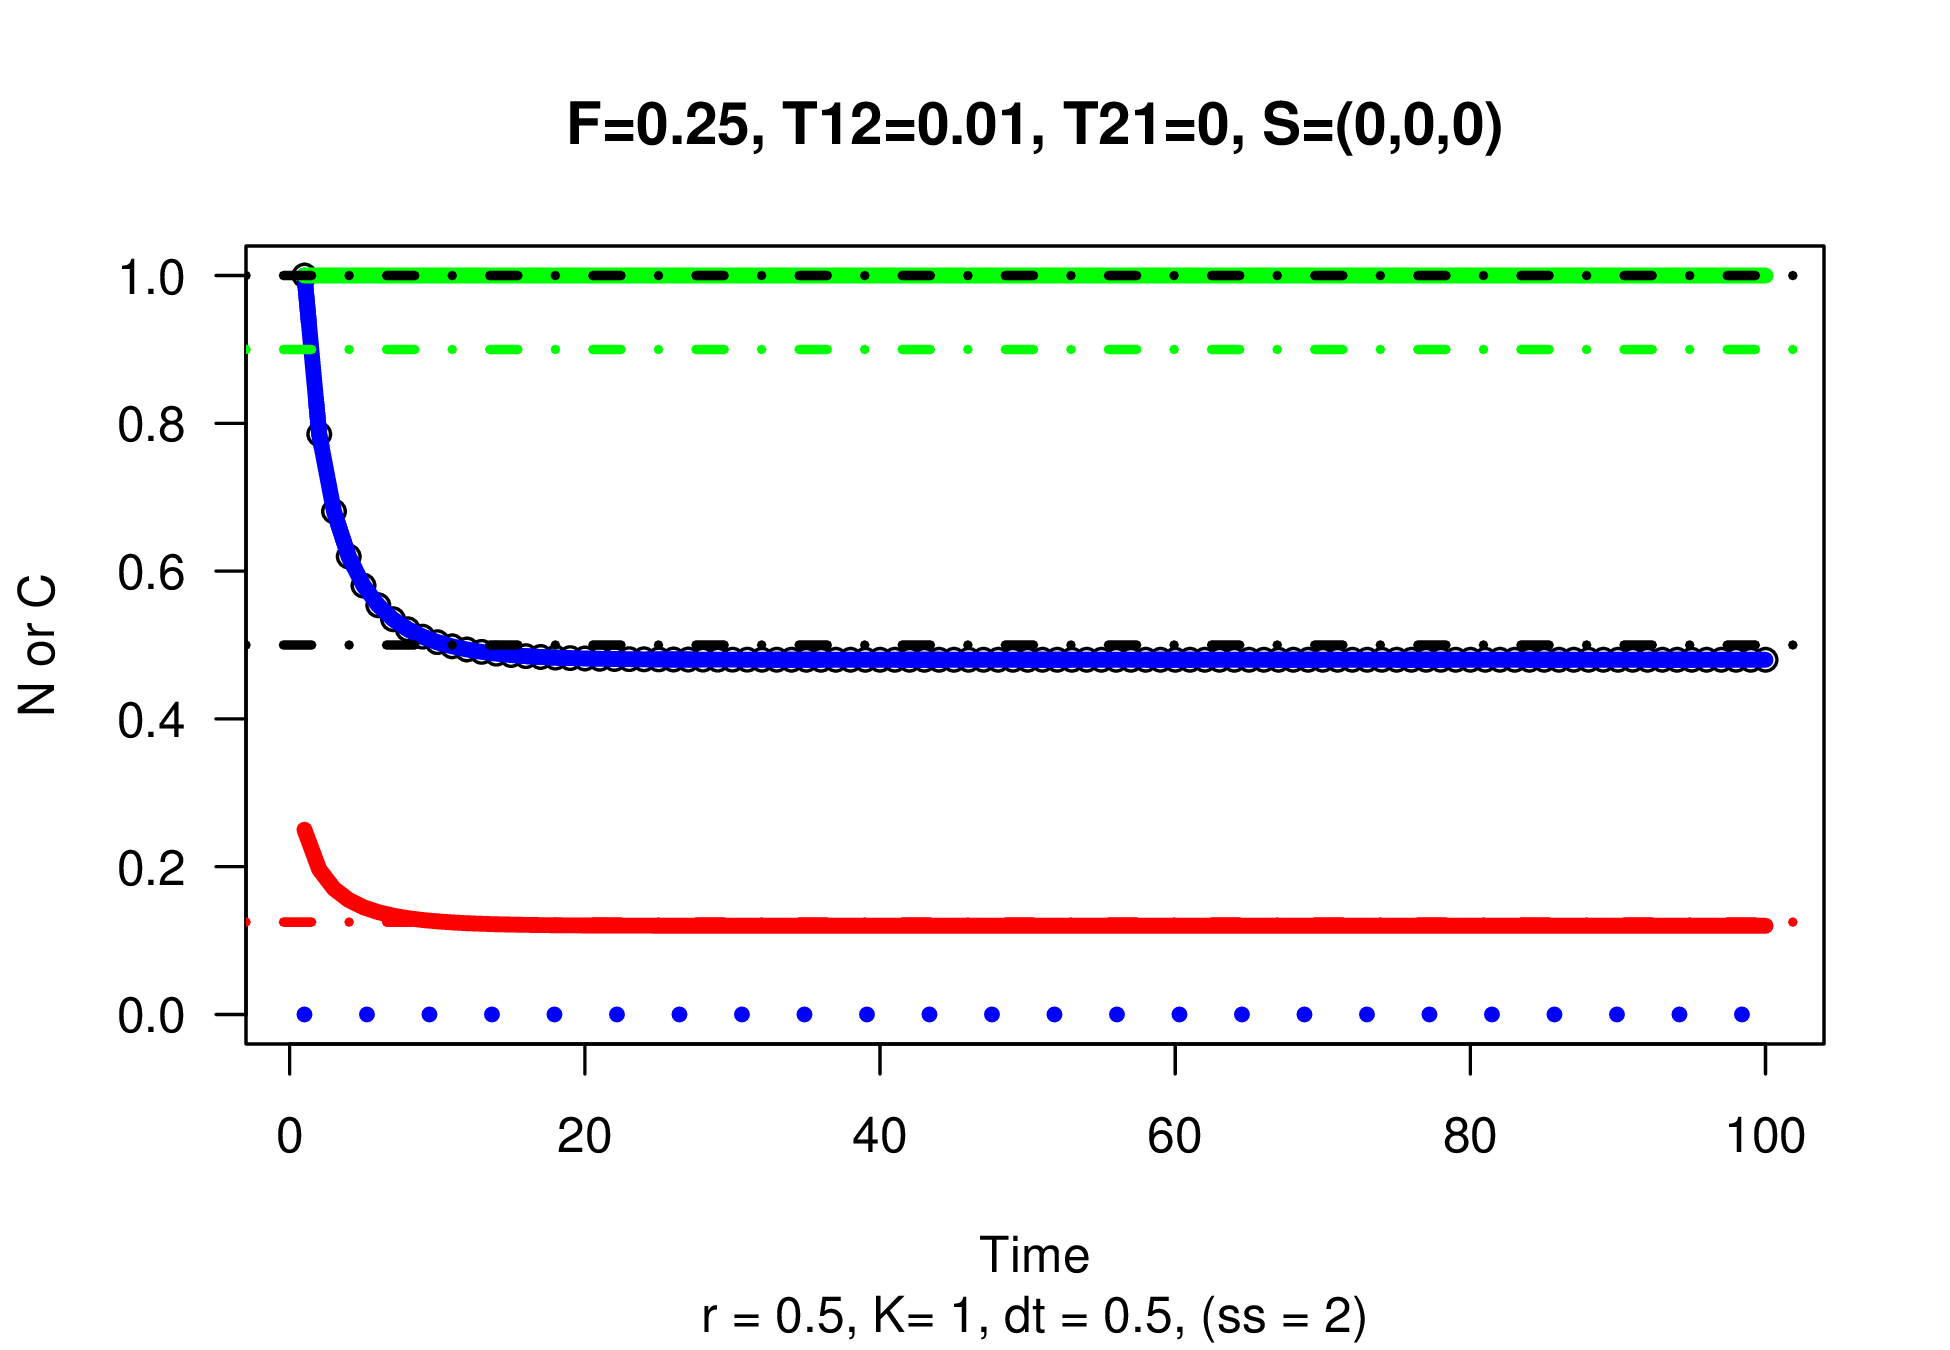
\includegraphics[height=0.5\textwidth]{./graphics/r05F025T12001T210S000.png}\\
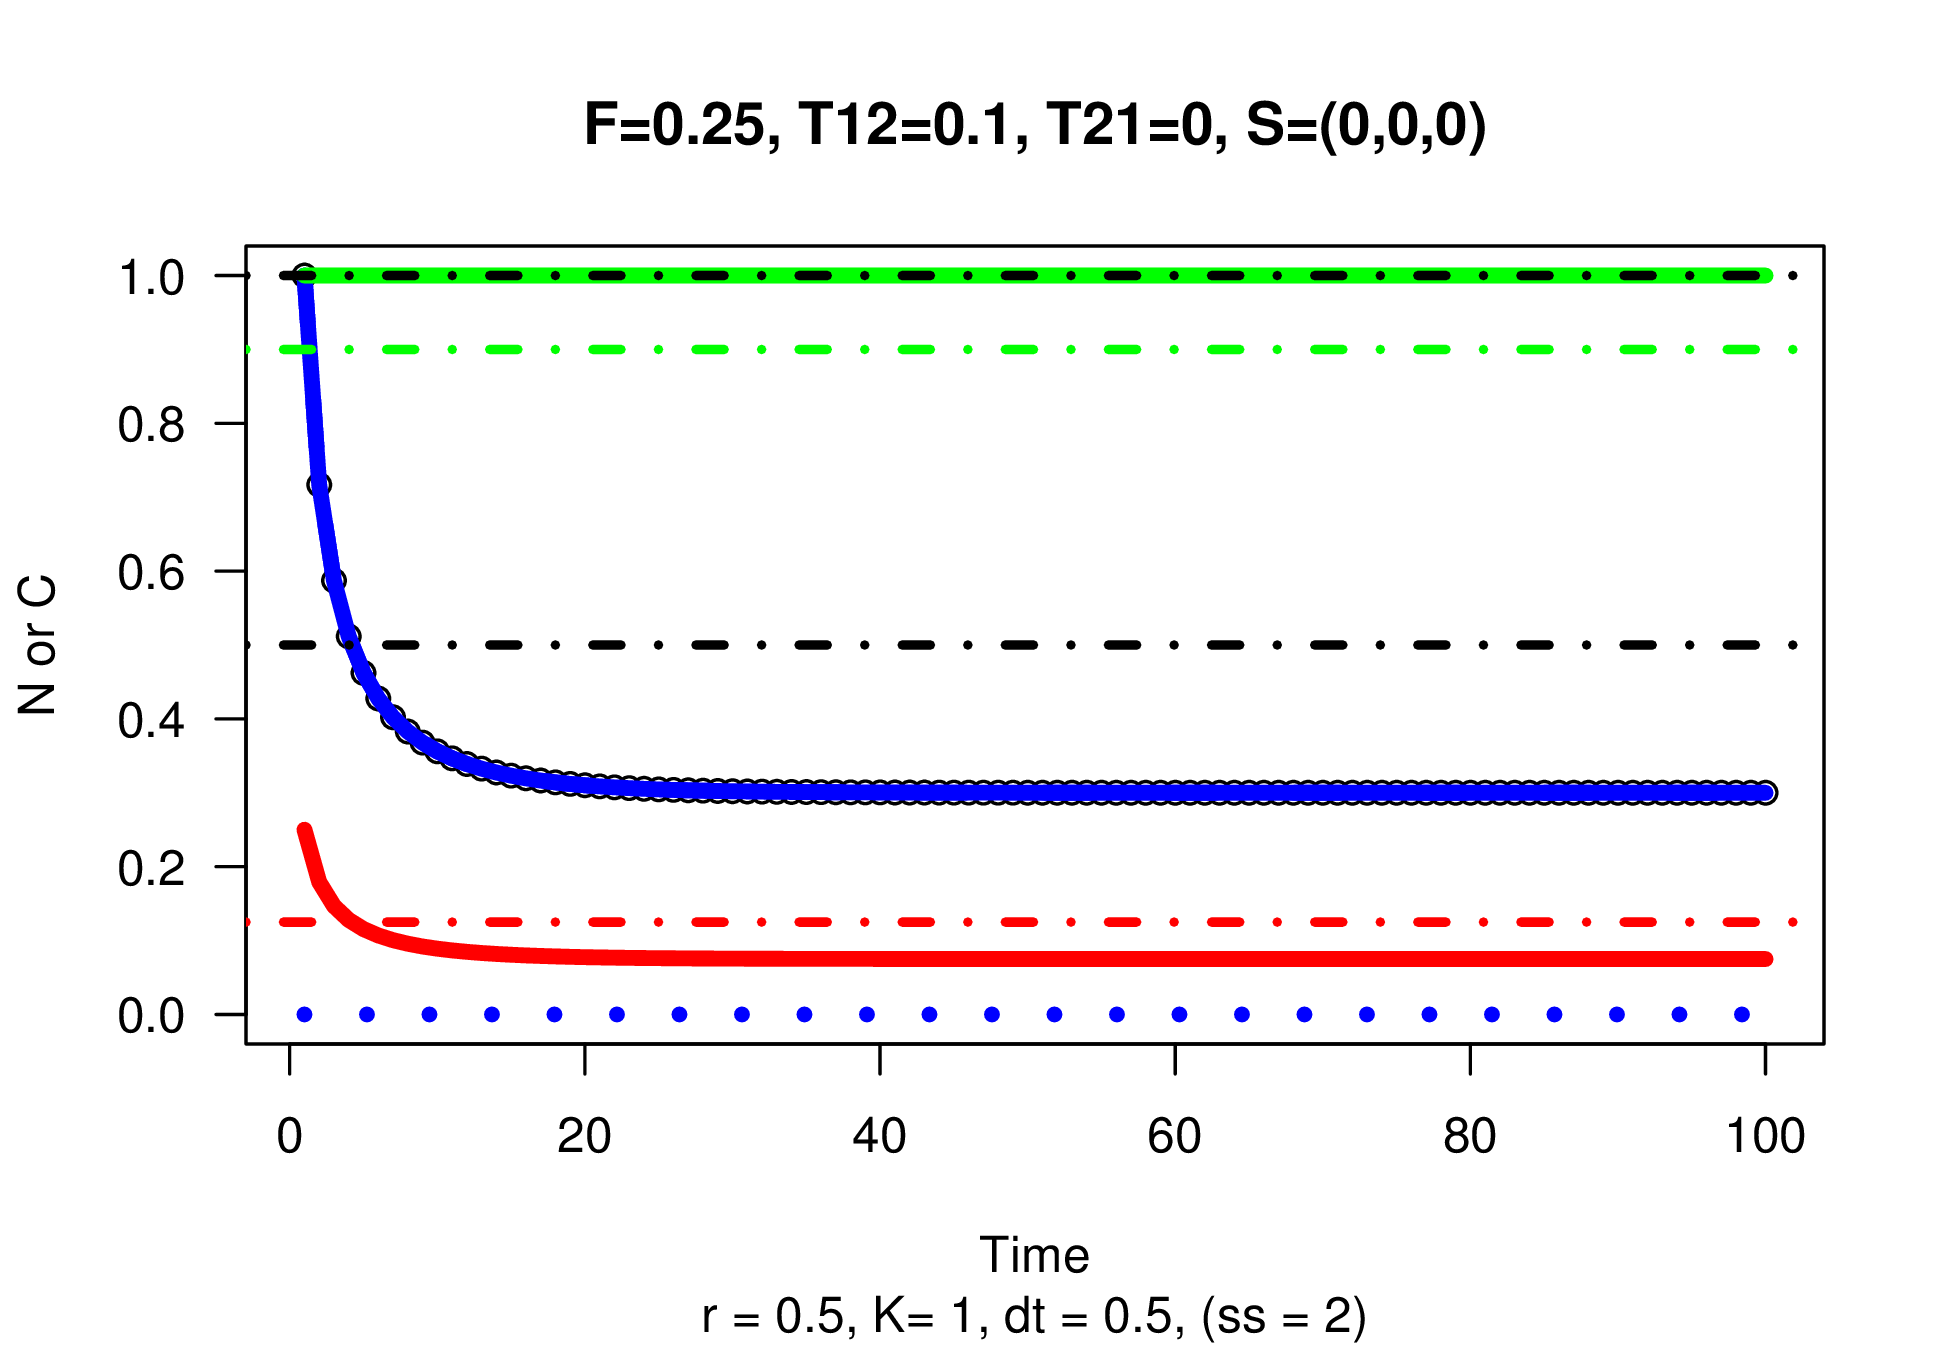
\includegraphics[height=0.5\textwidth]{./graphics/r05F025T1201T210S000.png}\\
\end{tabular}
\caption{\label{fig:emigration}
Effects if increasing levels of emigration,$T_{12} > 0; T_{21} = 0$.
As emigration increases, the size of the $\None$ population decreases, and
yield falls below MSY. Since there is no immigration, the
proportion local remains unchanged.
}
\end{center}
\end{figure}

\begin{figure}
\begin{center}
\begin{tabular}{c}
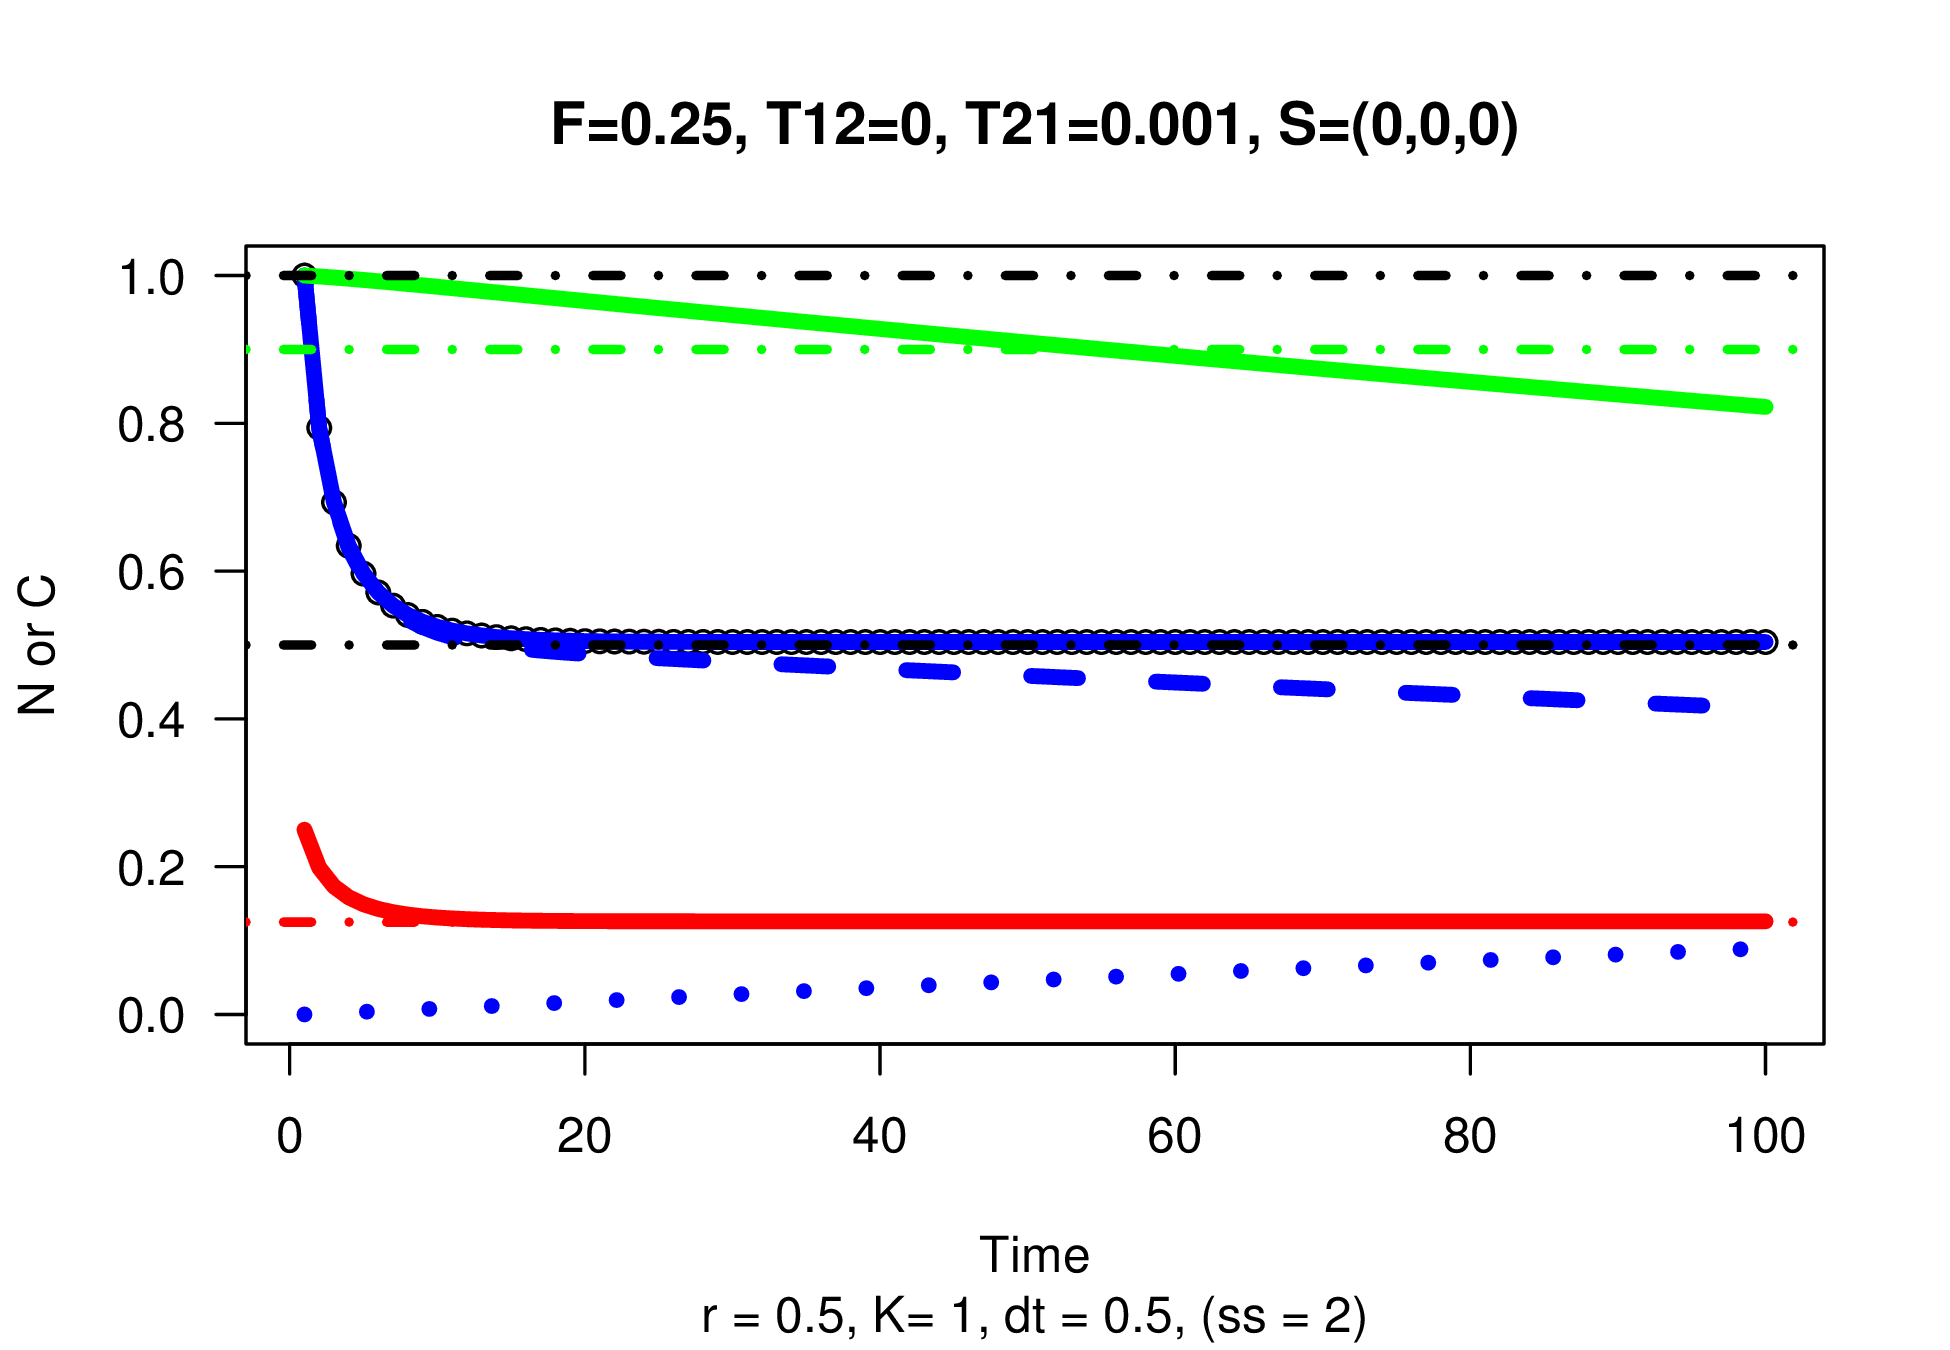
\includegraphics[height=0.5\textwidth]{./graphics/r05F025T120T210001S000.png}\\
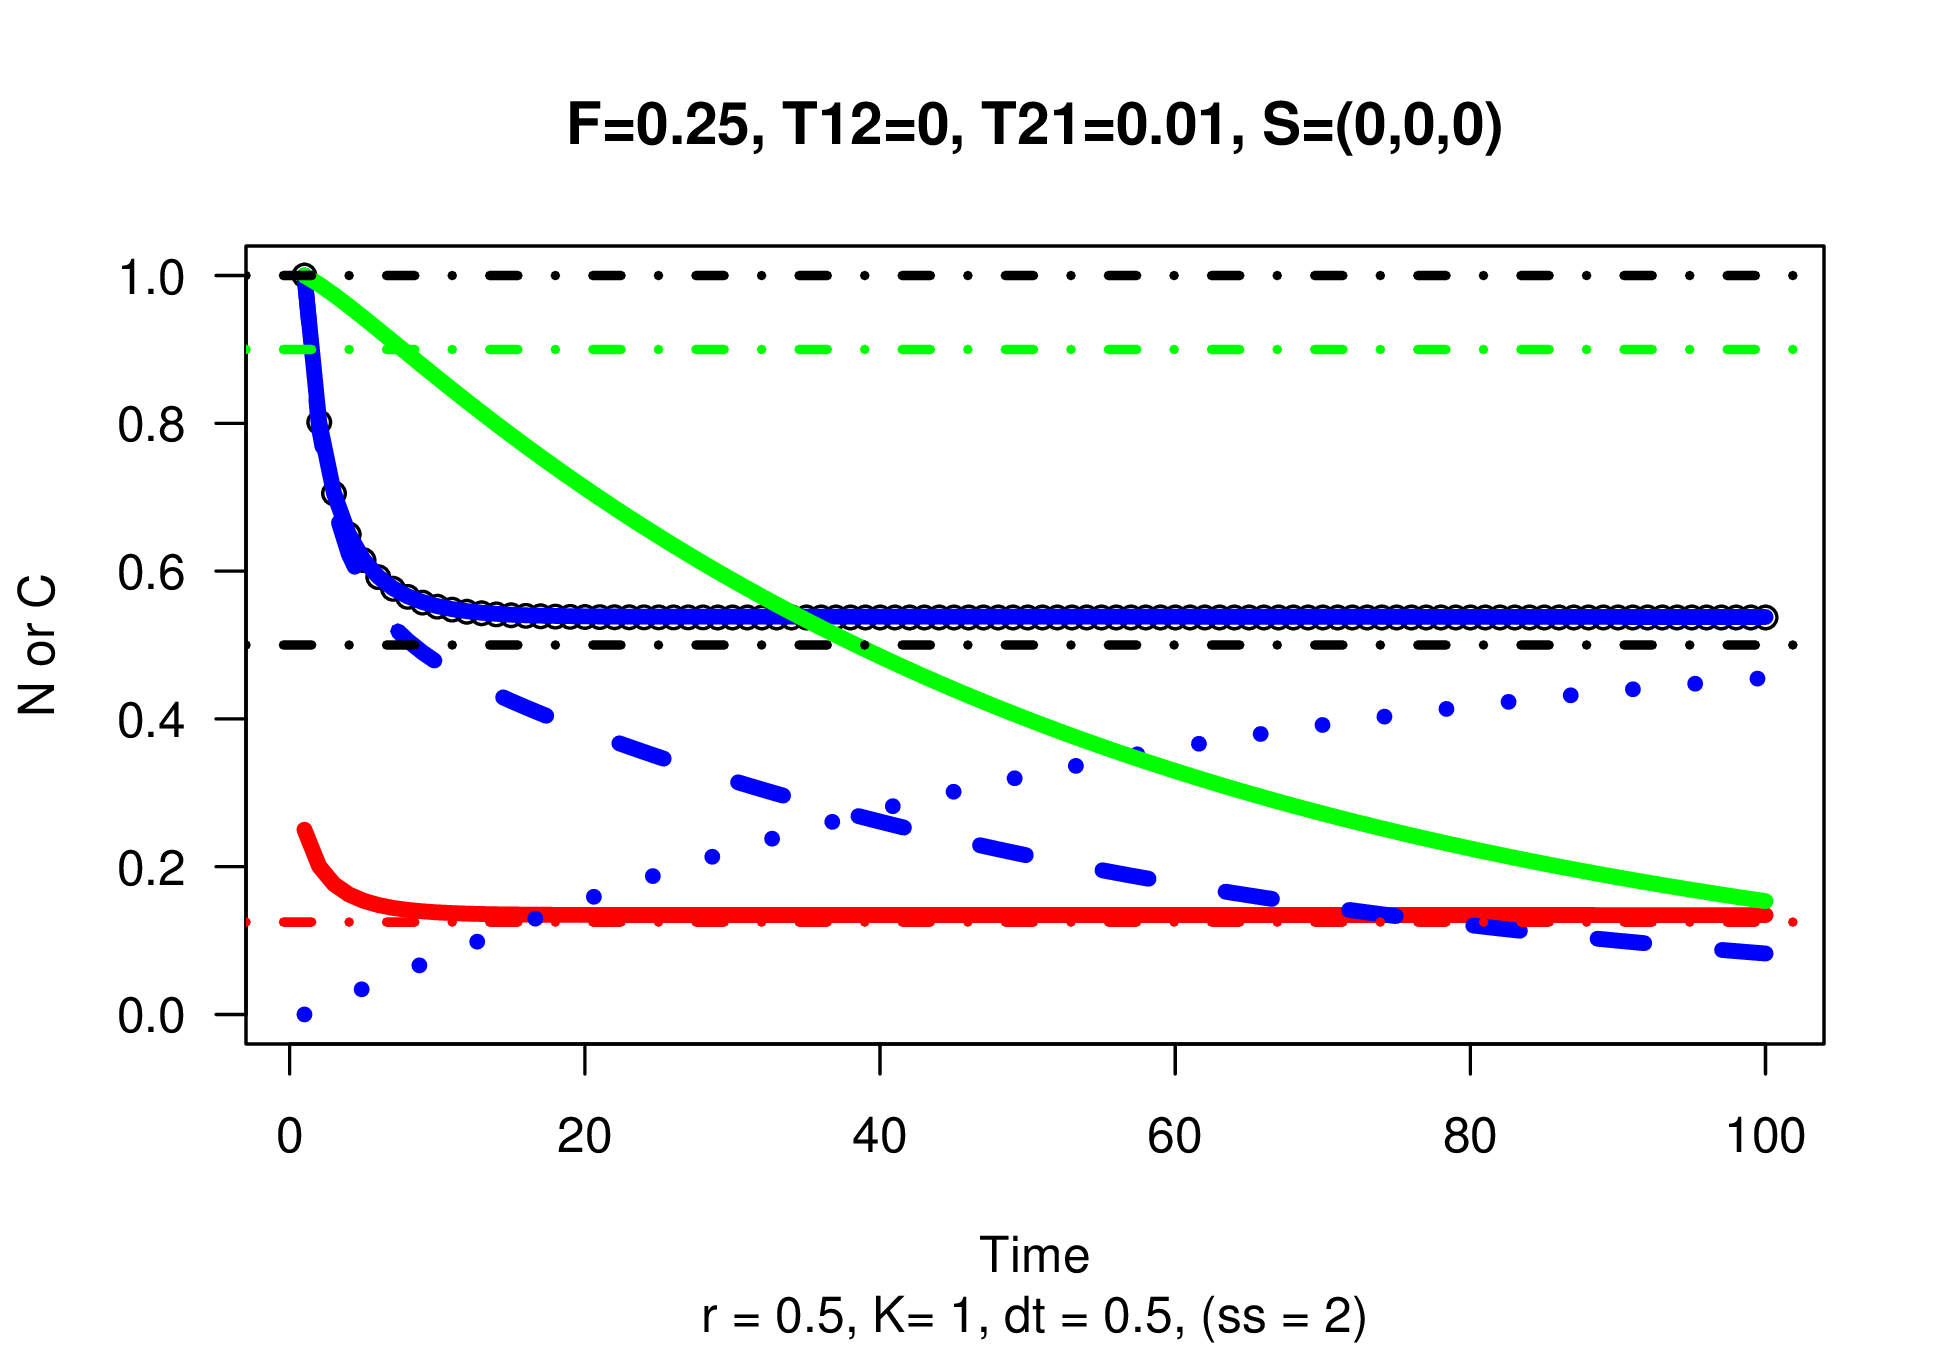
\includegraphics[height=0.5\textwidth]{./graphics/r05F025T120T21001S000.png}\\
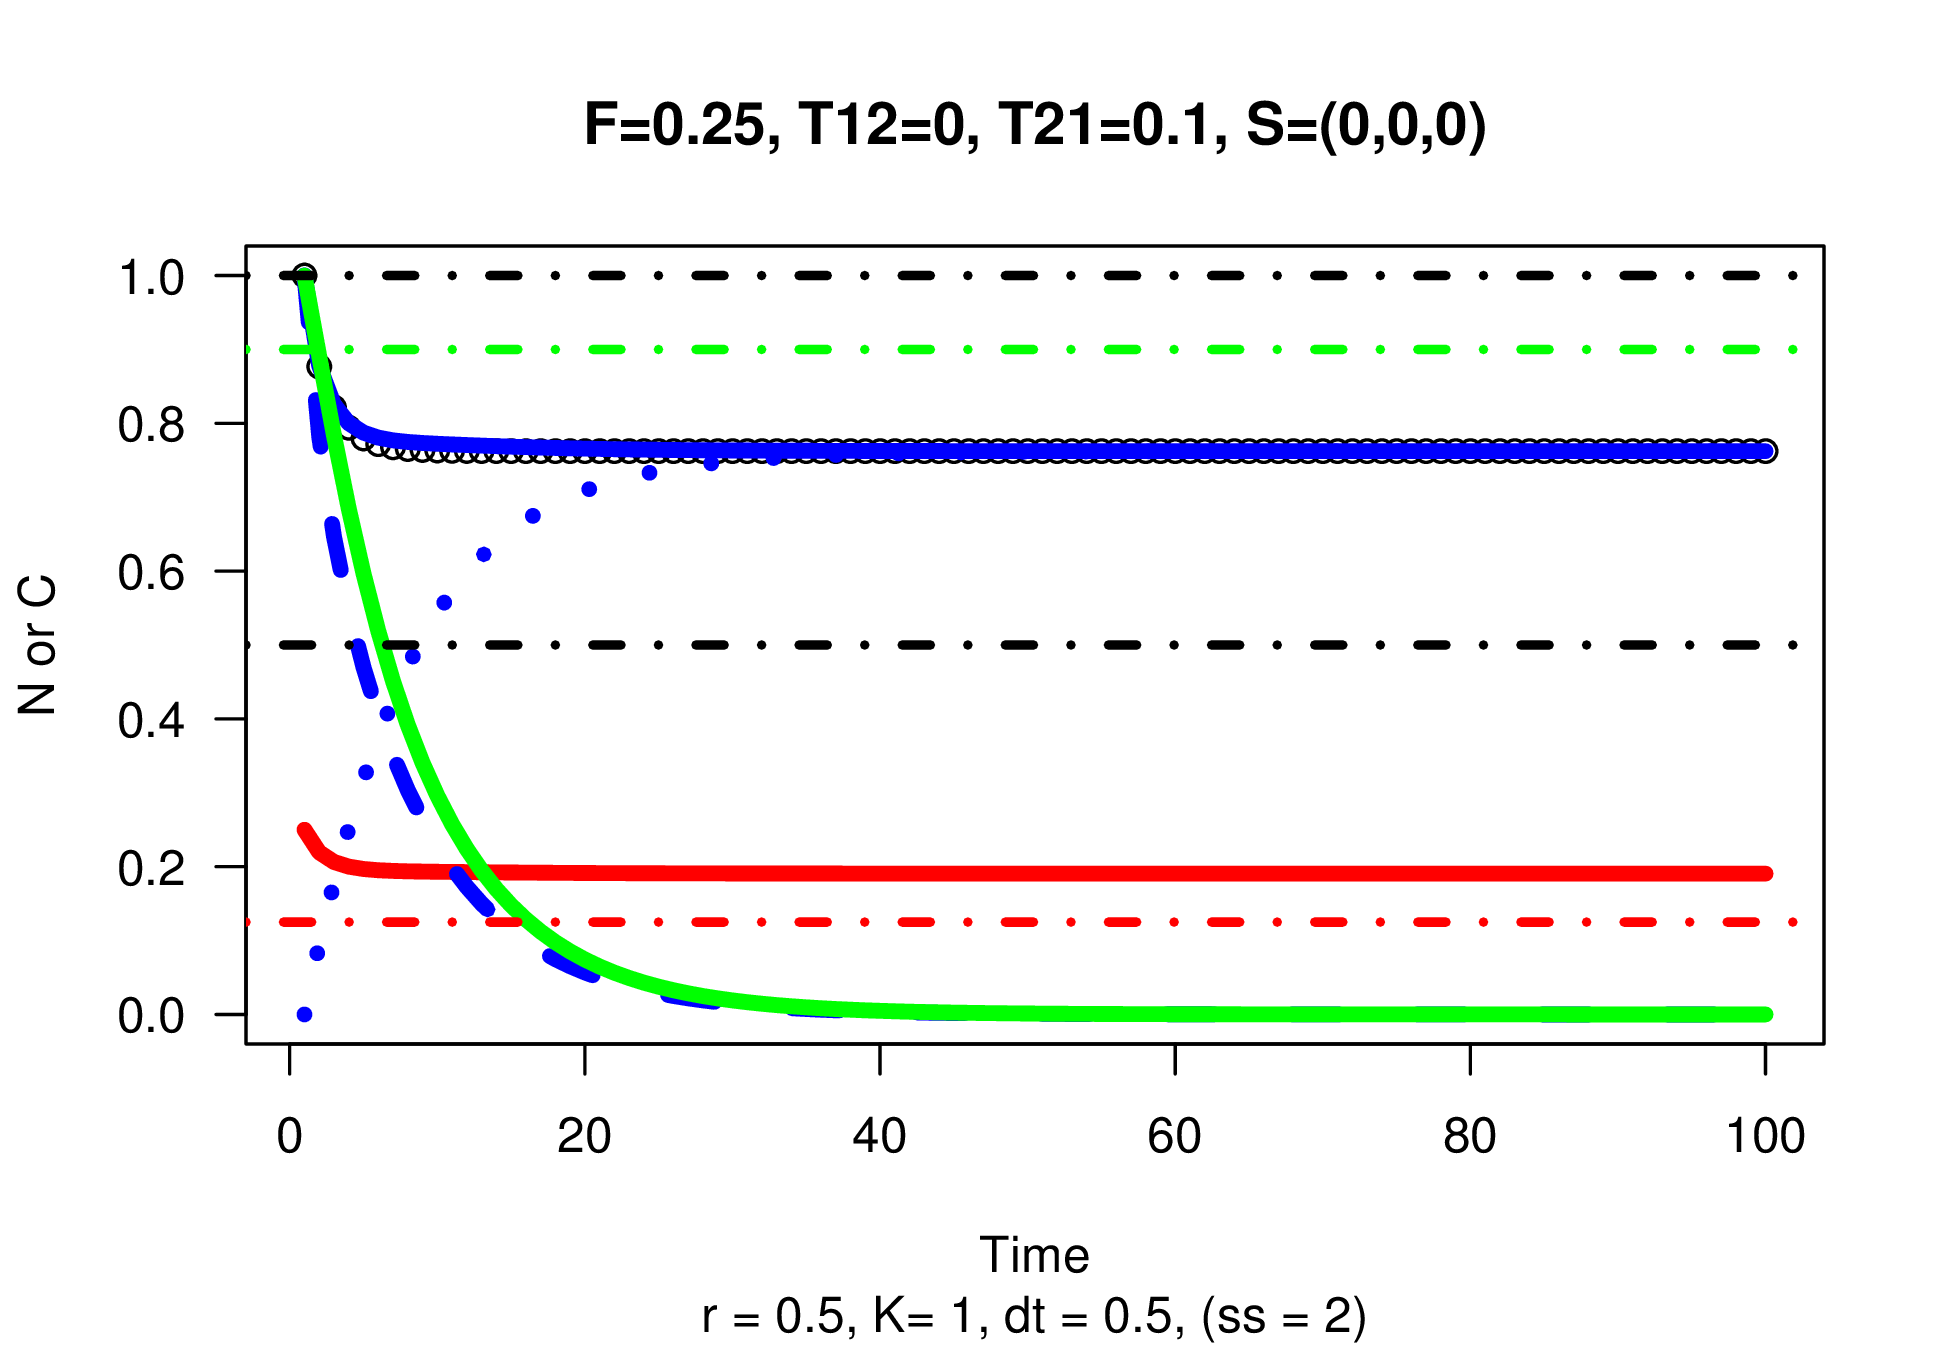
\includegraphics[height=0.5\textwidth]{./graphics/r05F025T120T2101S000.png}\\
\end{tabular}
\caption{\label{fig:immigration}
Effects if increasing levels of immigration,$T_{12} = 0; T_{21} > 0$.
As immigration increases, the size of immigrant population, $\Ntwo$,
increases (dotted blue line) and the proportion local declines well
below the 0.9 reference level. Yield exceeds MSY for the local stock.
}
\end{center}
\end{figure}


\begin{figure}
\begin{center}
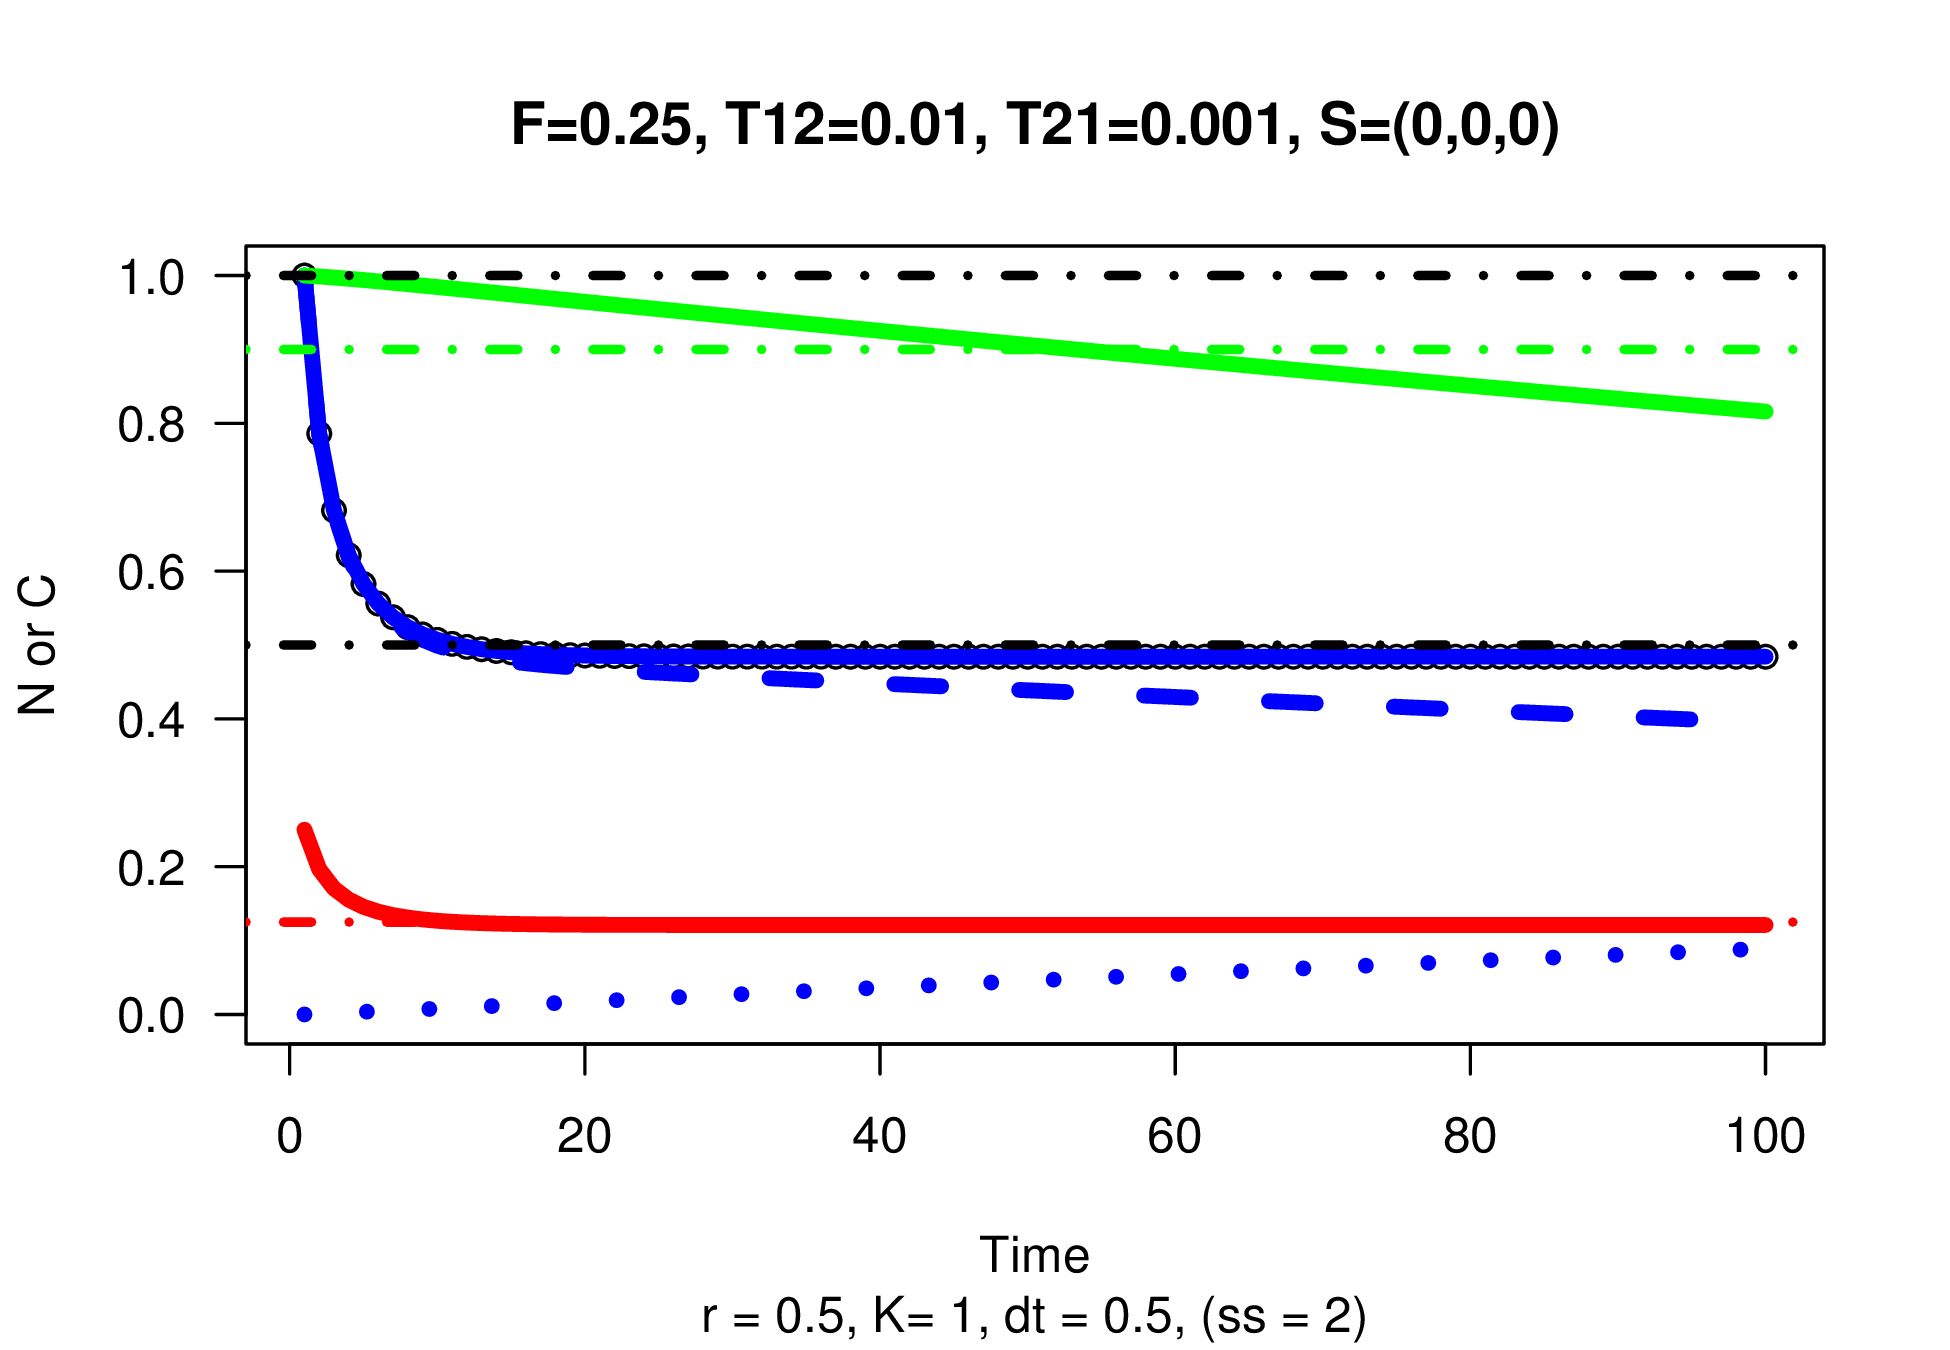
\includegraphics[height=0.7\textwidth]{./graphics/r05F025T12001T210001S000.png}\\
\caption{\label{fig:emandimm}
Effects of moderate levels of immigration and emigration. The local
population, $\None$, decreases and will eventually reach equilibrium
at $\None = 0$.
}
\end{center}
\end{figure}

\begin{figure}
\begin{center}
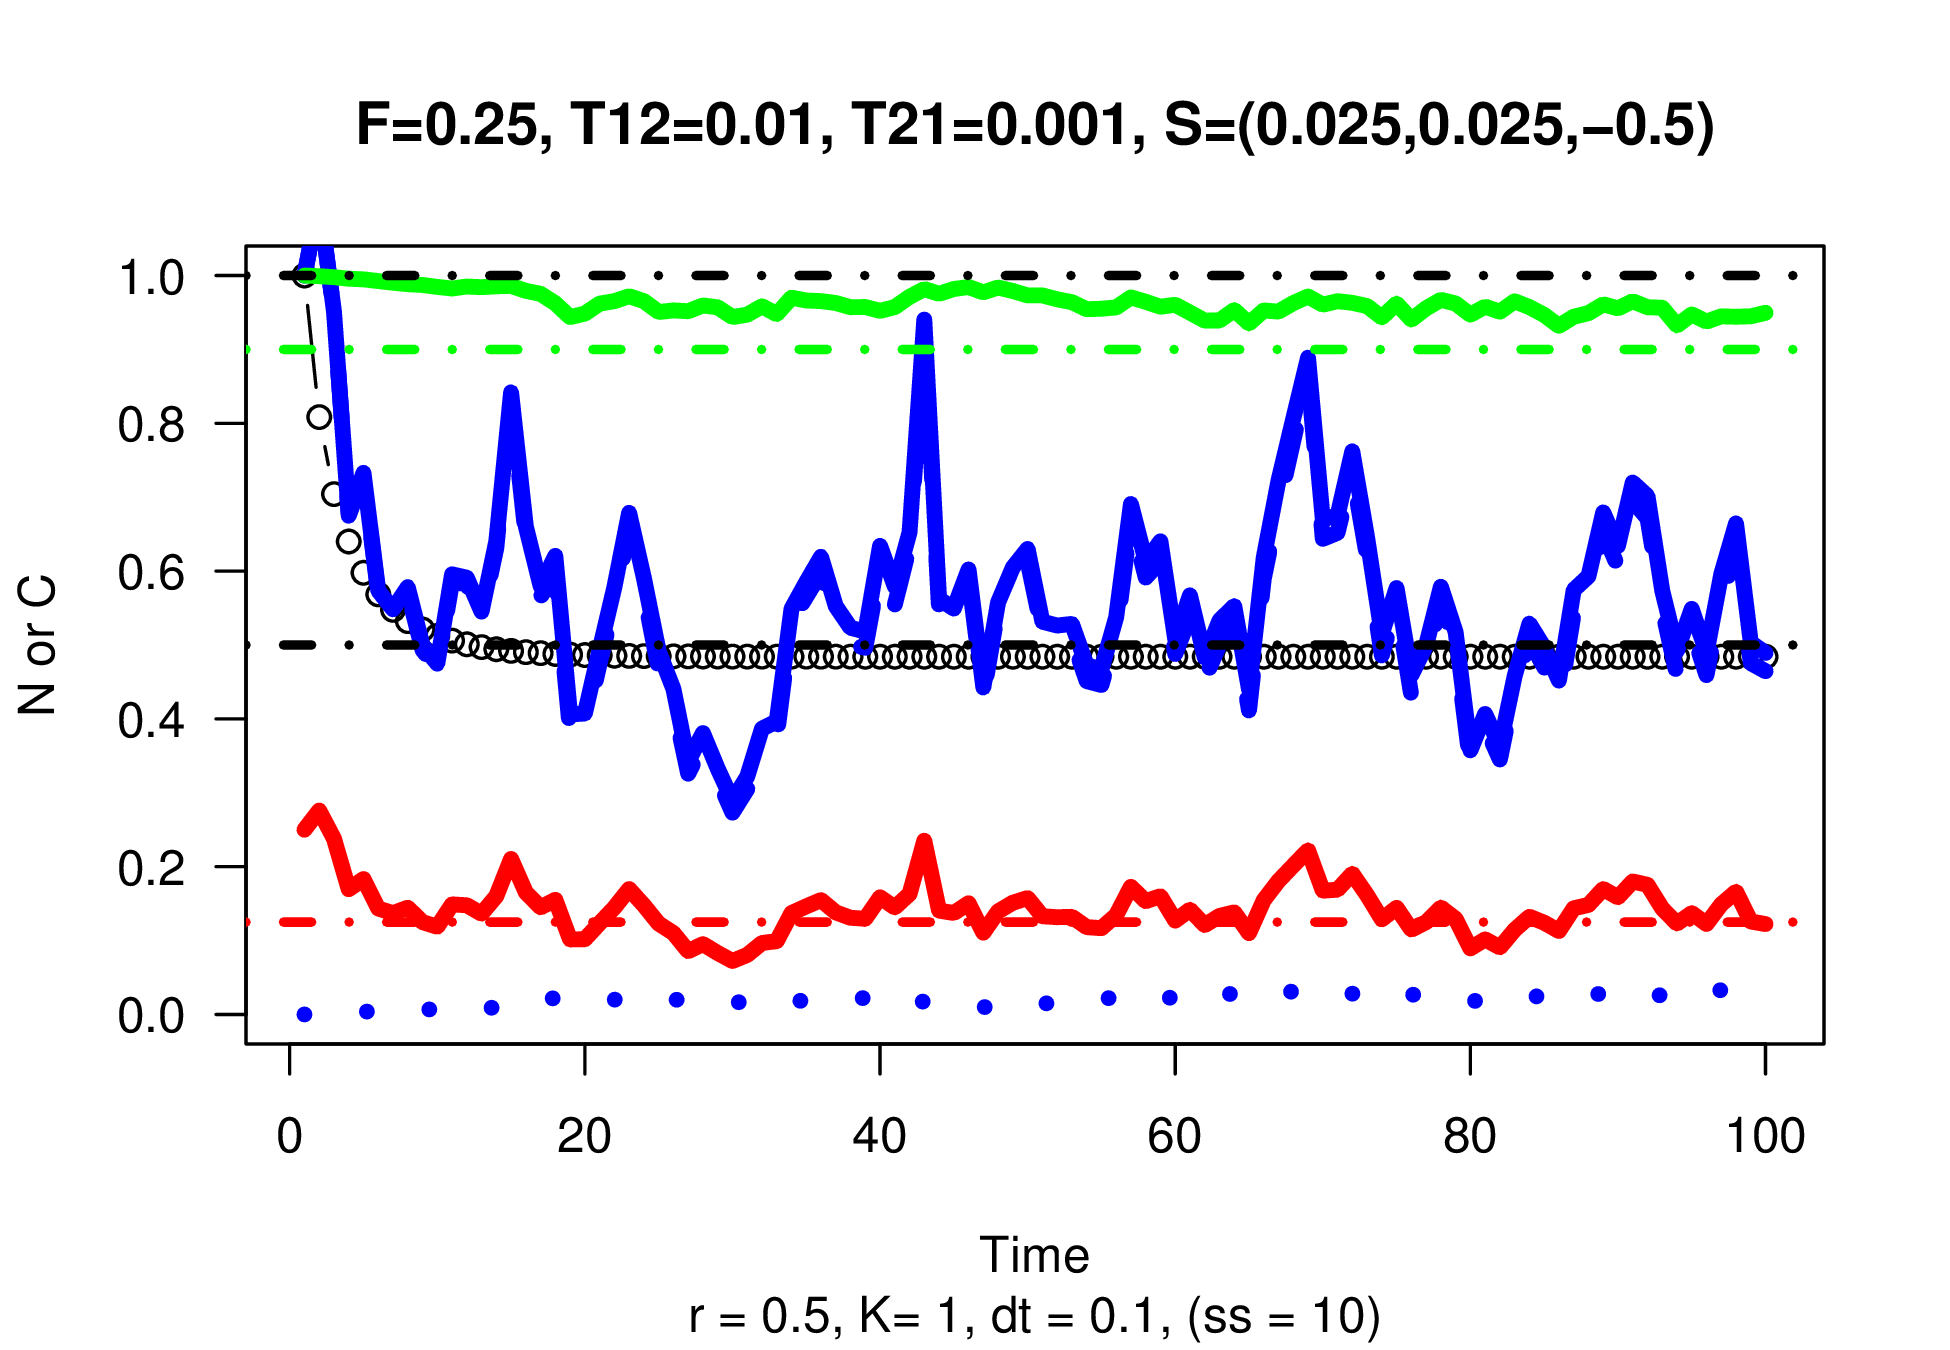
\includegraphics[height=0.7\textwidth]{./graphics/r05F025T12001T210001S00250025-05.png}
\caption{\label{fig:variance}
Effects of correlated random errors in the in $\None$ and $\Ntwo$ with
moderate levels of immigration and emigration.
Both populations appear to stabilize around some sort of steady
state size and the yield fluctuates around MSY.
}
\end{center}
\end{figure}

\end{document}
